\chapter{Results and Discussion}\label{ch:results_discussion}


\section{Results}\label{results}
In this section we present the results of our experiments. In the first part we will examine the overall results regarding reductive evolution before examining some other interesting findings in more detail.

\subsection{Genome Size}
In this section we will examine the results of the different conditions, focusing on which, if any, lead to a reduced genome. Figure~%TODO add figure showing genome size
presents the main findings regarding genome size. In the Figure, the blue line %TODO make sure the line is actually the blue one
represents the control condition and the other colors show the changed conditions: mutation up/down, selection up/down, and population up/down. As can be seen from the figure, 
\begin{figure}[H]
	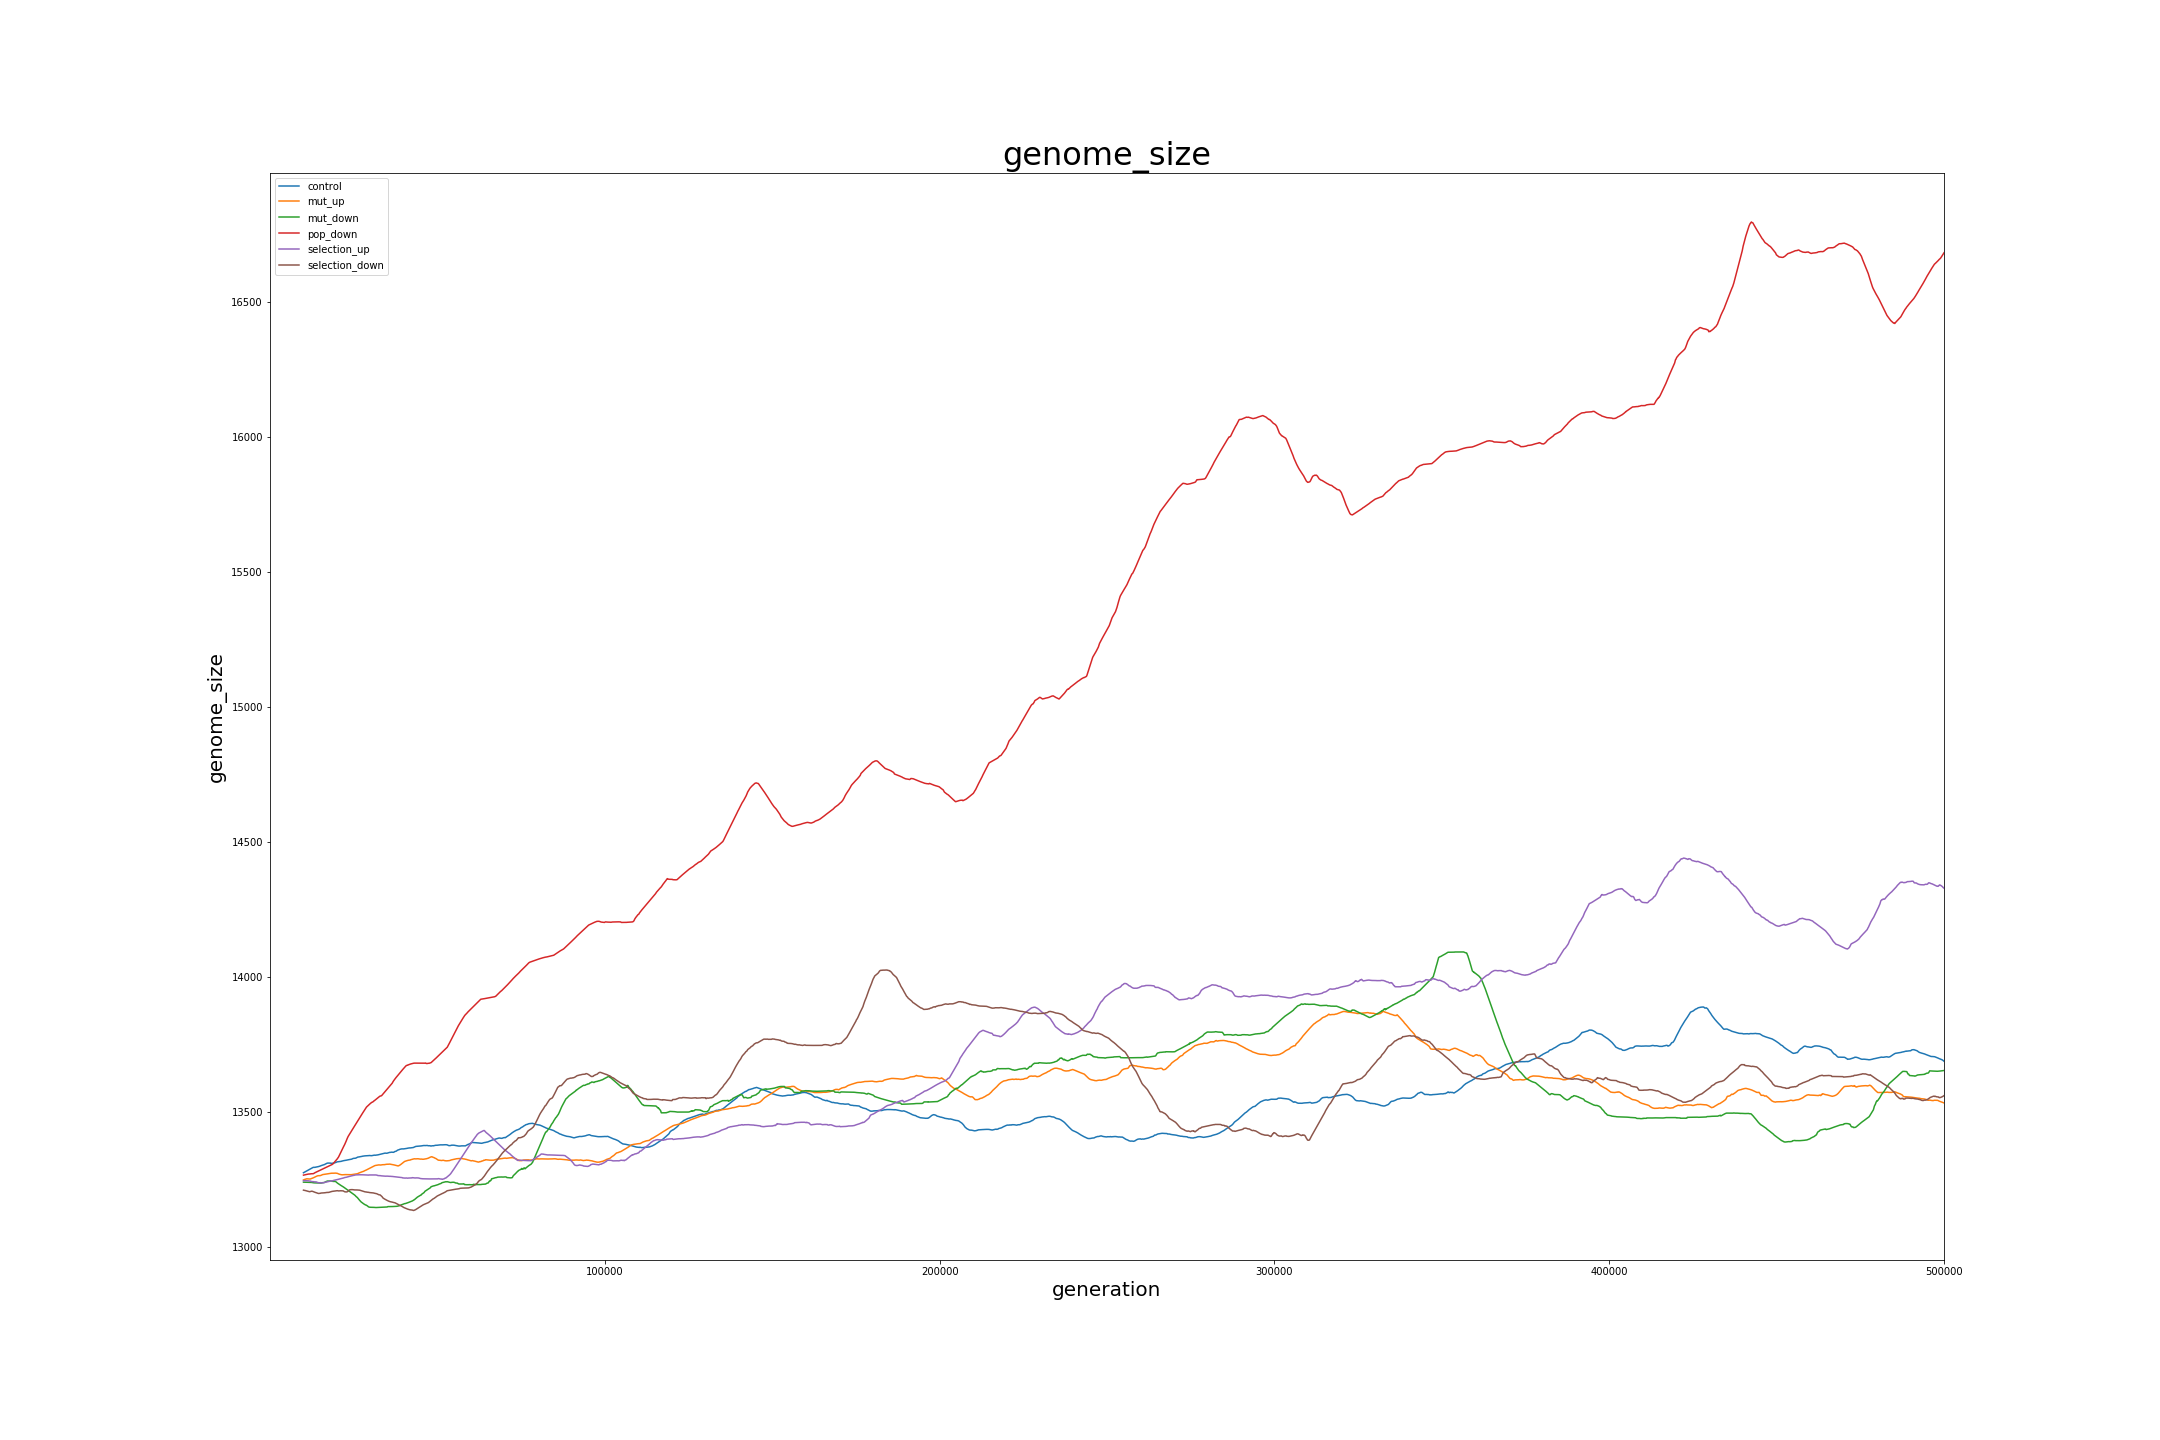
\includegraphics[width=\linewidth]{stat_fitness_mean_genome_size}
	\centering
	\caption[Genome size]{Genome size in number of bases of all conditions. Average taken across all five seeds for each condition.}
	\label{fig:genome_size}
\end{figure}
The most conspicuous observation is that none of the conditions resulted in a reduced genome size, and in fact the \textit{population down} condition had a runaway increase in the number of bases, reaching as high as 16,500 bases, a 25\% increase over the original wild type's roughly 13,200. Surprisingly, even after 500,000 generations it seems that the upper limit may still not have been reached. 

The next obvious observation is that of the remaining conditions, only the \textit{selection up} condition seems to have made much of a significant change with its 11\% increase. All of the remaining conditions had a mild increase in genome size. 


\subsection{Genome Structure}

\subsubsection{Noncoding DNA}

\subsubsection{Number of Genes}

\subsection{Evolvability}

\subsection{Robustness}


\section{Discussion}\label{discussion}

\subsection{Relation to Real-World Biological Entities}

\subsection{Limitations of Results}\label{limitations}
One limitation to consider is that only one parameter varied per condition. It may be possible that it is only under a combination of conditions (e.g. low selection \textit{and} high mutation rates) does reductive evolution occur. 

Another limitation is that the environments did not vary in our experiments. This could potentially have a large effect on robustness and evolvability, which are strong influencers of reductive evolution. 

Aevol as a modeling software is limited in that it relies, like all models, on several simplifications. The population sizes tested here, even in the population up condition, are still much smaller than would be found in real world populations. 